\subsection{Experiment 2: Model Selection in Cross-Validation}

The objective of this simulation experiment is to investigate the impact of improper model selection practices on evaluation bias. Two critical steps in the model selection process are considered: feature selection and hyperparameter tuning. The experiment hypothesizes that improper model selection — particularly the leakage of test set information during feature selection or hyperparameter tuning — will result in a significant overestimation of model performance.

To evaluate this hypothesis, three datasets are utilized: a null dataset with a baseline performance of  $r = 0$, a simulated spectral dataset, and a real spectral dataset. Feature selection is conducted by selecting the top 10 features most strongly correlated with the target variable, $y$. The original number of feature candidates varies across datasets, with 1000 for the null dataset, 300 for the simulated spectral dataset, and 18 for the real spectral dataset.

For hyperparameter tuning, the experiment employs a Support Vector Regression (SVR) model with two hyperparameters: the kernel function and the regularization parameter ($c$). The kernel functions considered are linear, sigmoid, and radial basis function (RBF), while the regularization parameter is set to two values: $c = 1.0$  and  $c = 0.01$. The kernel function determines how the selected features are transformed — either linearly or nonlinearly — to predict the target variable, $y$. The regularization parameter $c$ controls the trade-off between minimizing prediction error and model complexity; a larger $c$ allows for more error but reduces the likelihood of overfitting. In total, six SVR model variants (i.e., three kernel functions combined with two regularization parameter values) are available for selection during the evaluation process.

\begin{figure}[H]
    \centering
    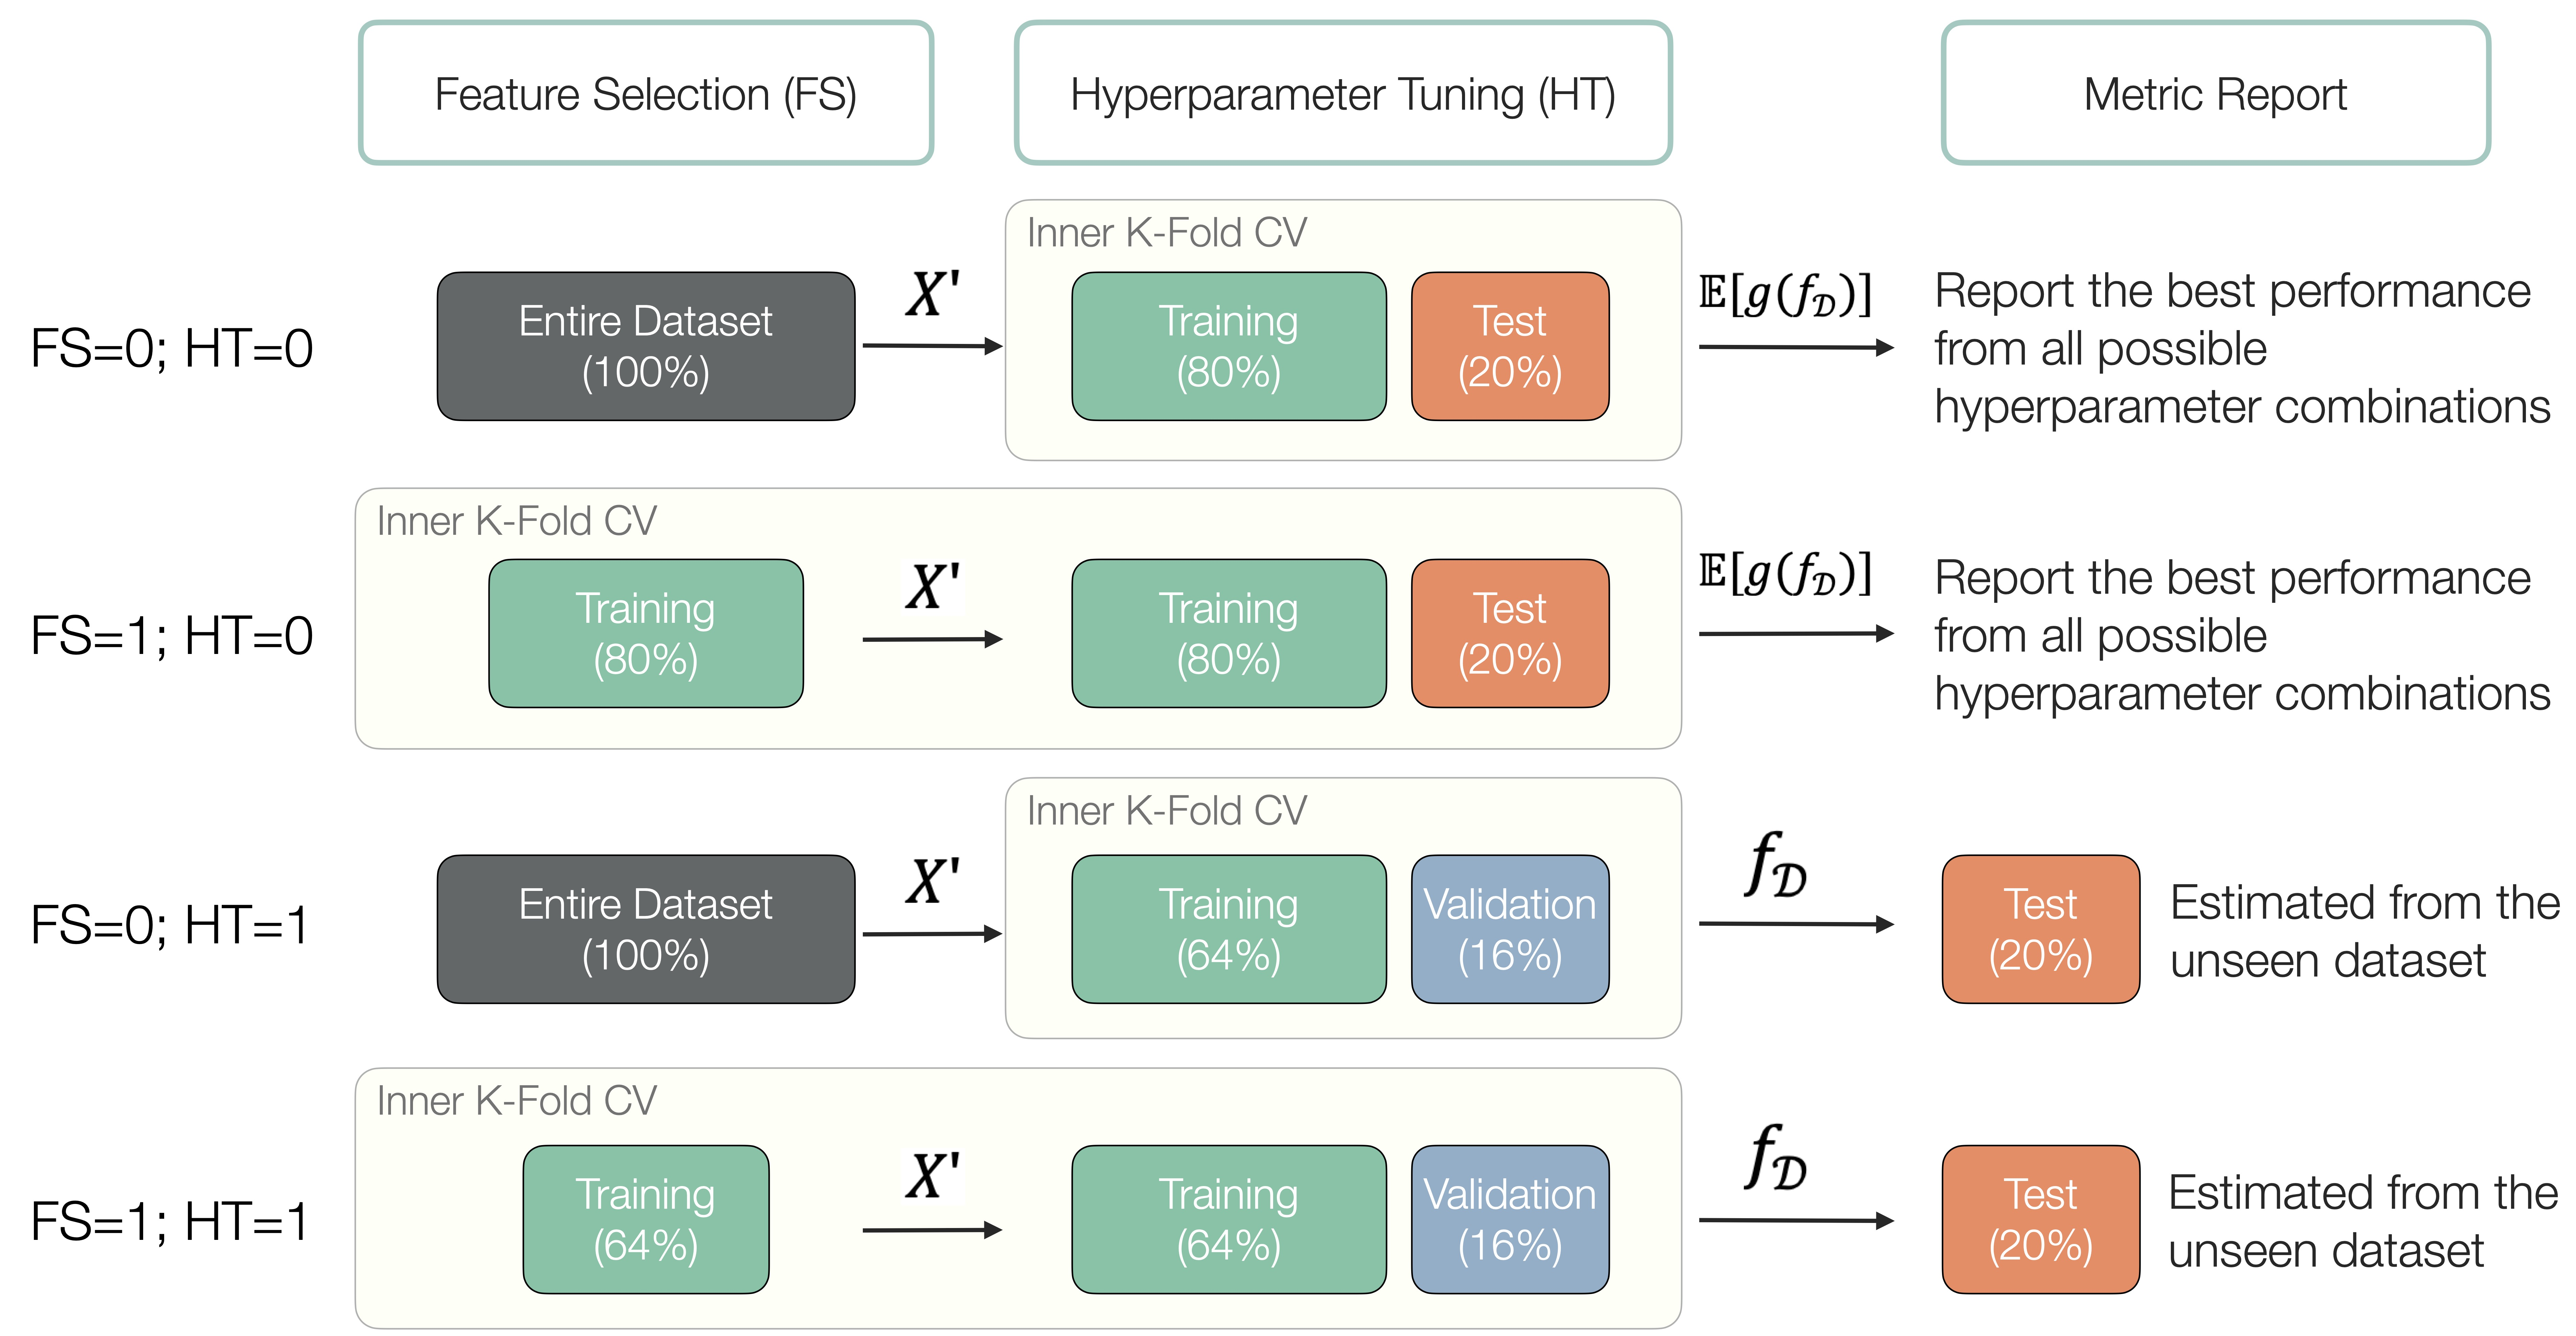
\includegraphics[width=1\textwidth]{fig_s2_schemes.jpg}
    \caption{Workflow diagram illustrating four cross-validation strategies of feature selection (FS) and hyperparameter tuning (HT), where 0 denotes incorrect implementation and 1 indicates correct practice. $X'$ is the selected feature subset, $\mathbb{E}[\hat{g}(f_\mathcal{D})]$ is the expected generalization performance, $f_\mathcal{D}$ is the model trained on the training set without being revealed to the test set.}
    \label{fig:s2_schemes}
\end{figure}

This experiment introduces notations FS for feature selection and HT for hyperparameter tuning, assigning a binary indicator (0 or 1) to denote incorrect (0) or correct (1) implementation of model selection. This yields four possible combinations of model selection strategies: “FS=0; HT=0”, “FS=0; HT=1”, “FS=1; HT=0”, “FS=1; HT=1” (Figure ~\ref{fig:s2_schemes}). When FS=0, feature selection precedes cross-validation splitting. If FS=1, feature selection occurs within each fold of the training set during cross-validation. With hyperparameter tuning, a correct implementation (HT=1) involves splitting the dataset into training (64\%), validation (16\%), and test (20\%) sets. The model is trained and tuned using the training and validation sets, respectively, while the test set is reserved for a single evaluation of model performance. Conversely, with HT=0, only training (80\%) and test (20\%) sets are used, risking evaluation bias as the test set informs both training and performance reporting. A 5-fold cross-validation approach was deployed for all strategies.
evaluation bias is measured as the discrepancy between the model selection-influenced performance estimate and the expected generalization performance (r=0), using the Pearson correlation coefficient between predicted and observed values. Over 500 sampling iterations, the experiment assesses the distribution of evaluation bias. A two-way analysis of variance (ANOVA) was conducted to examine the main effects of HT and FS on model performance. The ANOVA model was specified as $y \sim 1 + \text{HT} + \text{FS}$. This experimental setup is designed to quantify the extent of performance overestimation under improper model selection practices and provide insights into its implications for predictive modeling.